\documentclass[../piano-di-progetto.tex]{subfiles}
\begin{document}
\subsection{Progettazione della technology baseline}
Il periodo di progettazione della technology baseline inizia il 2020-04-21, dopo la revisione dei requisiti, e termina il giorno 2020-05-18 con la seconda revisione di avanzamento. 

\subsubsection{Ruoli}
Durante questa macro, viene richiesta la presenza dei seguenti ruoli:
\begin{itemize}
    \item Responsabile;
    \item Amministratore;
    \item Analista;
    \item Progettista;
    \item Verificatore.
\end{itemize}

\subsubsection{Attività}   
Per semplicità, questa macro viene suddivisa in periodi:
\begin{itemize}

    \item \textbf{I periodo (2020-04-21 - 2020-04-22)}:
        \begin{itemize}
            \item Revisione ed eventuale aggiornamento dei seguenti documenti:
            \begin{itemize}
                \item \textsc{Norme di progetto v1.0.0};
                \item \textsc{Analisi dei requisiti v1.0.0};
                \item \textsc{Piano di progetto v1.0.0};
                \item \textsc{Piano di qualifica v1.0.0}.
            \end{itemize}

            \item \textbf{Verifica}
        \end{itemize}

    \item \textbf{II periodo (2020-04-23 - 2020-04-26)}:
        \begin{itemize}
            \item \textbf{Ricerca degli strumenti}: studio autonomo degli strumenti richiesti per lo sviluppo del progetto; 
            \item \textbf{Progettazione}: progettazione dell'architettura di sistema;
            \item \textbf{Verifica}.
        \end{itemize}
    \item \textbf{III periodo (2020-04-27 - 2020-05-10)}: vengono effettuati quattro incrementi per la realizzazione di un \glossario{proof of concept}, verranno illustrati nella prossima sottosezione.
    \item \textbf{IV periodo (2020-05-11 - 2020-05-18)}: 
            \begin{itemize}
                \item \textbf{Preparazione della presentazione};
                \item \textbf{Verifica}.
            \end{itemize}
        \end{itemize}
\subsubsection{Incrementi}

\paragraph{I incremento}
\textbf{2020-04-27 - 2020-05-29}. 
 
 Vengono stabiliti i seguenti obiettivi per l'incremento:
 \begin{itemize}
     \item Installazione e configurazione di Grafana;
     \item Installazione e configurazione dell'ambiente di sviluppo \glossario{Electron}.
 \end{itemize}

Durante l'incremento verranno svolte le seguenti attività: 
\begin{itemize}
    \item Progettazione;
    \item Codifica;
    \item Verifica;
\end{itemize}

\paragraph{II incremento}
\textbf{2020-04-30 - 2020-05-02}. 
 
 Vengono stabiliti i seguenti obiettivi per l'incremento:
 \begin{itemize}
     \item Creazione del \glossario{front-end} del programma di addestramento.
 \end{itemize}

Durante l'incremento verranno svolte le seguenti attività: 
\begin{itemize}
    \item Progettazione;
    \item Codifica;
    \item Verifica.
\end{itemize}


\paragraph{III incremento}
\textbf{2020-05-03 - 2020-05-06}. 
 
 Vengono stabiliti i seguenti obiettivi per l'incremento:
 \begin{itemize}
     \item Implementazione della logica applicativa per l'input dei dati nel programma di addestramento;
     \item Implementazione dell'algoritmo di RL per la generazione dei \glossario{predittori} nel programma di addestramento.
 \end{itemize}

Durante l'incremento verranno svolte le seguenti attività: 
\begin{itemize}
    \item Progettazione;
    \item Codifica;
    \item Verifica.
\end{itemize}


\paragraph{IV incremento}
\textbf{2020-05-07 - 2020-05-10}. 
 
 Vengono stabiliti i seguenti obiettivi per l'incremento:
 \begin{itemize}
     \item Implementazione del front-end del plug-in per la visualizzazione dei dati in grafici e indici;
 \end{itemize}

Durante l'incremento verranno svolte le seguenti attività: 
\begin{itemize}
    \item Progettazione;
    \item Codifica;
    \item Lettera di presentazione;
    \item Consuntivo di periodo;
    \item Verifica.
\end{itemize}



\newpage
\begin{landscape}
    \begin{figure}[H]
        \centering
        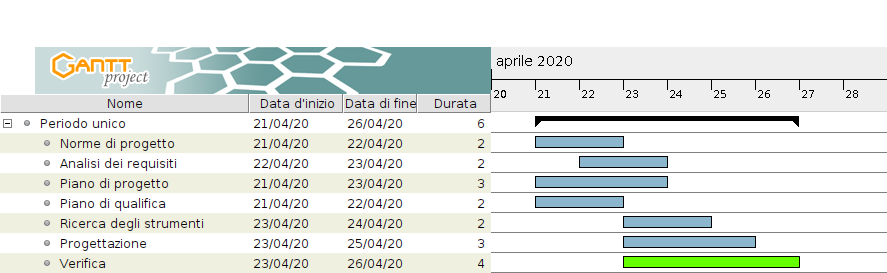
\includegraphics[width=24cm]{img/progettazione.png}
        \caption{Diagramma attività nel periodo di progettazione della technology baseline}
      \end{figure}
\end{landscape}

\end{document}
